\documentclass{standalone}
\usepackage{tikz}
\begin{document}
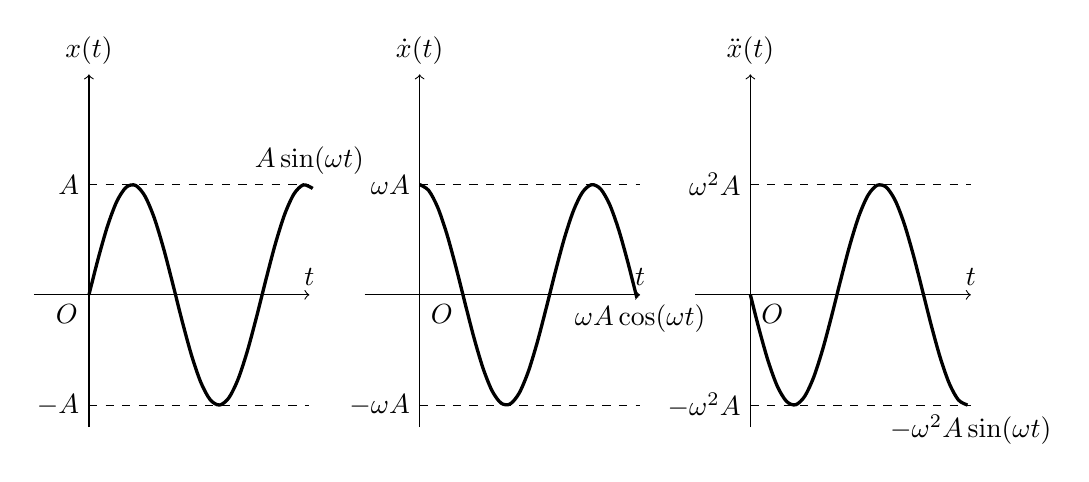
\begin{tikzpicture}[scale=1.4]

    \node[below] at (-3.2,0) {$O$};
    \draw[->] (-3.5, 0) -- (-1, 0) node[above]{$t$};
    \draw[->] (-3,-1.2)--(-3,2)node[above]{$x(t)$};
    \draw[very thick] plot[smooth, domain=-3:-0.97] (\x, {sin(4*(\x+3) r)});
    \draw[dashed] (-3,1) node[left] {$A$} -- (-1,1) node[above]{$A\sin(\omega t)$};
    \draw[dashed] (-3,-1) node[left] {$-A$} -- (-1,-1);


    \node[below] at (0.2,0) {$O$};
    \draw[->] (-0.5, 0) -- (2, 0) node[above]{$t$}node[below]{$\omega A\cos(\omega t)$};
    \draw[->] (0,-1.2)--(0,2)node[above]{$\dot x(t)$} ;
    \draw[very thick] plot[smooth, domain=0:1.97] (\x, {cos(4*\x r)});
    \draw[dashed] (0,1) node[left] {$\omega A$} -- (2,1);
    \draw[dashed] (0,-1) node[left] {$-\omega A$} -- (2,-1);

    \node[below] at (3.2,0) {$O$};
    \draw[->] (2.5, 0) -- (5, 0) node[above]{$t$};
    \draw[->] (3,-1.2)--(3,2)node[above]{$\ddot x(t)$};
    \draw[very thick] plot[smooth, domain=3:4.97] (\x, {-sin(4*(\x-3) r)});
    \draw[dashed] (3,1) node[left] {$\omega^{2} A$} -- (5,1);
    \draw[dashed] (3,-1) node[left] {$-\omega^{2} A$} -- (5,-1)node[below]{$-\omega^{2}A\sin(\omega t)$};

\end{tikzpicture}
\end{document}